%!TEX root = thesis.tex
\chapter{Background} \label{ch:background}

In this chapter, we introduce laser scanning and the 3D-reconstruction pipeline. In section~\ref{sec:heritage} we describe our problem's heritage preservation context. In section~\ref{sec:scanners} we introduce 3d scanning followed by the process by which raw scanner data transformed into a model in section~\ref{sec:pipeline}. We then discuss the cleaning process in section~\ref{sec:cleaning}.




\section{Digital heritage preservation} \label{sec:heritage}

Architectural heritage sites in many parts of the world are under threat of deterioration and destruction especially in developing countries. There is a need to preserve these heritage sites due to their historical relevance, if not physically, at least digitally. The demolition of  the Buddhas of Bamiyan by the Taliban in 2001 \cite{Toubekis2009} is one illustration of this need. Preservation efforts have utilised various technologies to record historical sites. Early efforts used tape measures and theodolites to produce simple ground plans. More recently photogrammetry let geomaticians produce 3D models \cite{Heritage}. Now laser range scanners allow us to create extremely high resolution 3D models.


\section{3D scanning} \label{sec:scanners}

There is an enormous variety of 3D scanners in the market today. Each scanner has properties that make it more of less suitable for various scanning tasks. Generally the size of the object and the level of detail one wishes to capture dictates the technology. The imaging speed, portability and cost or a scanner is also considered.

Scanning technologies can generally be classified into 2 categories, namely triangulation and time of flight scanners.

\subsection{Triangulation scanners}

\begin{figure}[H]
	\begin{subfigure}[b]{.33\textwidth}
	  \centering
	  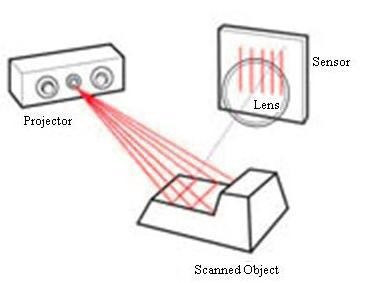
\includegraphics[width=.9\linewidth]{images/structured-light-scan}
	  % \caption{Structured light 3D scanning \cite{Form2014}}
	  % \label{fig:structured-light-scan}
	\end{subfigure}%
	\begin{subfigure}[b]{.33\textwidth}
	  \centering
	  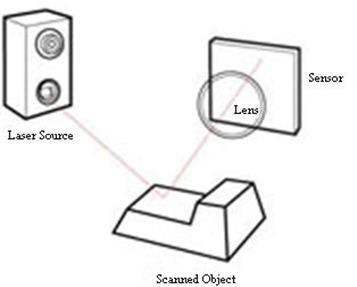
\includegraphics[width=.9\linewidth]{images/triangulate-laser-scan}
	  % \caption{Laser 3D scanning}
	  % \label{fig:images/triangulate-laser-scan}
	\end{subfigure}
	\begin{subfigure}[b]{.33\textwidth}
	  \centering
		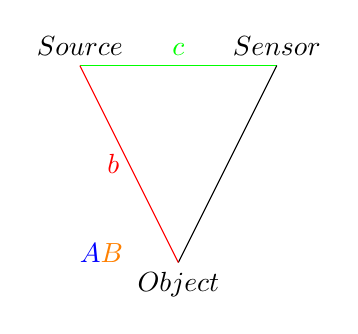
\begin{tikzpicture}[scale=2.5]

		\coordinate [label={[black]above:$Source$}] (A) at (0, 1);
		\coordinate [label={[black]above:$Sensor$}] (B) at (1, 1);
		\coordinate [label={[black]below:$Object$}] (C) at (0.5, 0);

		\draw[green] (A) -- node [above] {$c$} (B);
		\draw[black] (B) -- node [right] {$ $} (C);
		\draw[red] (C) -- node [left] {$b$} (A);

		\tkzMarkAngle[fill=white, size=0.25cm,%
		opacity=1](C,A,B)
		\tkzLabelAngle[pos=0.15](C,A,B){$\color{blue}A$}

		\tkzMarkAngle[fill=white,size=0.25cm,%
		opacity=1](A,B,C)
		\tkzLabelAngle[pos=-0.15](C,B,A){$\color{orange}B$}

		% \tkzMarkAngle[fill=green,size=0.25cm,%
		% opacity=.4](B,C,A)
		% \tkzLabelAngle[pos= 0.15](B,C,A){$ $}

		\end{tikzpicture}
	\end{subfigure}
	\caption{Triangulation 3D scanners}
	\label{fig:triangulation-scanners}
\end{figure}

Triangulation scanners, as the name suggests, uses trigonometric triangulation to locate a point in a scene relative to scanner. Triangulation can be performed by either emitting a laser point, line or by projecting a series of linear patterns and then picking up the reflection with a sensor at a known position. During laser triangulation, the displacement of the object affects the angle at which the laser is returned (see \autoref{fig:triangulation-scanners}). Using structured light, the distortions in the patterns from the sensor's perspective can be used to determine the angle of reflected light \cite{Brown2012}. Given the precise distance between the light source and sensor ($\begingroup\color{green}c\endgroup$) and as well as the outgoing angle of emitted light ($\begingroup\color{blue}A\endgroup$) and incoming angle of reflected light ($\begingroup\color{orange}B\endgroup$), the distance to the object is given by $\begingroup\color{red}b\endgroup = \begingroup\color{green}c\endgroup\frac{ sin(\begingroup\color{orange}B\endgroup)}{sin(\pi - \begingroup\color{blue}A\endgroup-\begingroup\color{orange}B\endgroup)}$.

\subsection{Time of flight scanners (TOF)}

\begin{figure}[ht]
  \centering
  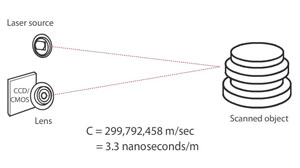
\includegraphics[width=.5\linewidth]{images/pulse-tof}
  \caption{Time of flight scanner}
  \label{fig:tof}
\end{figure}

Time of flight scanners emit laser pulses and measure the time it takes for a pulse reflection to be detected by the scanner's sensor (see \autoref{fig:tof}). Given the speed of light the distance traveled by the light can be determined. Given the time it takes to for light to travel to a surface and back to the scanner ($t$), the distance ($d$) can is given by $d = ct/2$ where $c$ is the speed of light. The accuracy of the distance calculation depends on how precisely time can be measured \cite{Form2014}.

\begin{figure}[b]
	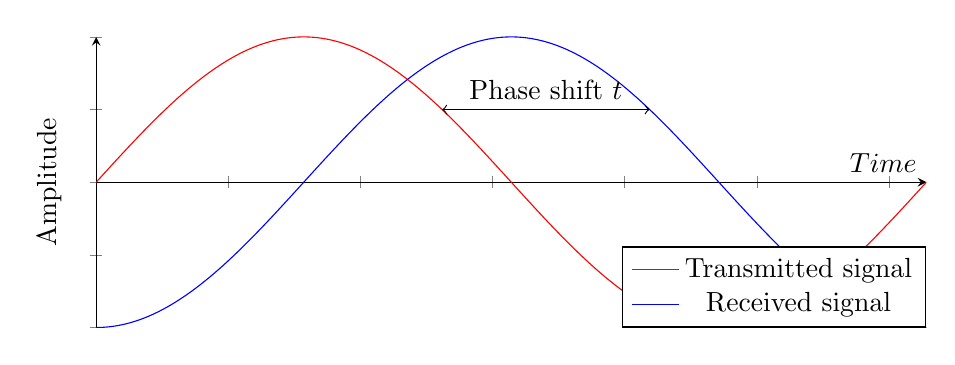
\begin{tikzpicture}[scale=1]
	\begin{axis}[
		width=1\textwidth,
		height=150,
	    axis lines = left,
	    yticklabels={,,},
	    xticklabels={,,},
	    axis x line=center,
	    xlabel = $Time$,
	    ylabel = {Amplitude},
	    legend style={
	    at={(1,0)},
	    anchor=south east}]
	]
	\addplot[samples=500,domain=0:2*pi, color=red]{sin(deg(x))};
	\addlegendentry{Transmitted signal}
	\addplot[samples=500,domain=0:2*pi, color=blue]{sin(deg(x-pi/2))};
	\addlegendentry{Received signal}
	\draw[<->] (axis cs:2.61799,0.5) -- node[above]{Phase shift $t$} (axis cs:4.18879,0.5);
	\end{axis}
	\end{tikzpicture}
	\caption{Phase shift in returned signal}
	\label{fig:phase-shift}
\end{figure}

Laser phase-shift scanners is a variation on the standard TOF scanner. These scanners modulate the power of the laser pulse in a sinusoidal wave during a scan. The phase shift in the returning pulse is used to the round trip time (see \autoref{fig:phase-shift}). Due to the cyclical nature of the signal, phase shift is ambiguous. This ambiguity is resolved by using measurements at multiple frequencies \cite{Bhurtha}.



\subsection{Comparison}

Triangulation scanners can achieve 10 micrometer accuracy over distances less than one meter. Over longer distances the triangle in \autoref{fig:triangulation-scanners} becomes to long and the distance calculation error prone. Structured light scanners tend to be faster than laser scanners as the whole scene is captured instead of a single point at a time \cite{Brown2012}. Light scanners scanners are also less prone to motion distortions. Hand held scanners of this type exists which reduces setup time compared to other scanners.

Time of flight scanners can time a round trip of a laser pulse to an object more accurately over long distances than triangulation scanners can estimate perspective distortions. This technology does however not deal well with distances less than 2 meters. Pure TOF scanners can scan distances up to 1000 meters \cite{Form2014}. TOF scanners can be set to sample at different resolutions. Low resolution scans (10 000 points) may take seconds while higher resolution scans (millions of points) may take minutes.

Phase based scanners are more limited in range due to the ambiguity of returned signals from beyond the design distance \cite{Bhurtha}. Objects from beyond the scanner's designed range can sometimes be found at closer distances when the scanner software fails to discard far away points. Phase based scanners make up for this shortfall by being much faster and more accurate within its range \cite{Form2014}. T


\begin{table}
\begin{tabular}{ |l|l|l|l|l|l| }
  \hline
  Type &              Range &        Precision       & Speed & Portability \\
  \hline
  Structured light &    <1m     & 10 micrometer  & Seconds & High \\
  Laser triangulation & <1m     & 10 micrometer  & Seconds  & Medium \\     
  TOF &                 2-1000m & Medium      & Minutes & Low \\
  Phase &               2-100m & Low         & Seconds to Minutes & Low \\
  \hline  
\end{tabular}
\caption{Comparison of scanning technology}
\end{table}


\subsection{Data}

The terrestrial laser scanners as described above all produce angle and range measurements that are converted into 3D coordinates relative to the scanner. In addition to that scanners also record the intensity of the light returned. High end scanners sometimes have integrated cameras that are used to map colors to captured data points. Orientation and GPS measurements are also available in some models which help speed up registration (discussed later).

Scanner manufacturers may keep lower level measurements that are specific to their scanners. This data may valuable in cleaning artifacts from scans. However, lower level data tend to be locked away in propriety formats which are not accessible to us. We therefore limit our investigation to data that can be readily exported from scanner software. We also do not consider color information as such datasets were not readily available to us.

% (Mention non uniform point density somewhere? too obvious?)
% (Mention scanner resolution increasing over time?)

\subsection{Artifacts}

Besides the phase binning issues with phase based TOF scanners, there are many more limitations that one should be aware of. Due to the optical nature of the above scanners, difficulties are often encountered when dealing with shiny, mirroring or transparent objects. Windows cannot be captured as light passes through without being reflected. Mirror like surfaces also go missing because light does not reflect back towards the scanner. The sun and other bright objects and cause points not associated with any physical object to appear in a scan. Fog and smoke can also cause problems.

\begin{figure}[ht]
  \centering
  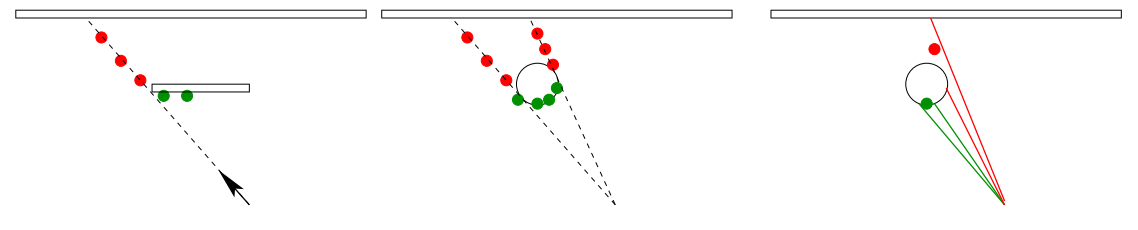
\includegraphics[width=1\linewidth]{images/mixed-pixel}
  \caption{Mixed pixels. Green are valid points and red are not. \cite{Tuley2005}}
  \label{fig:mixed-pixel}
\end{figure}

Mixed pixels is another problematic aspect of laser scanning. When a laser pulse partially hits a near and then subsequently a far object, the result is a data point between the near and far object \cite{Tuley2005} (see \autoref{fig:mixed-pixel}).


\pagebreak


Time of flight scanners are generally used in the cultural heritage domain because of their long range. These scanners will be the focus of our research.


\section{3D reconstruction pipeline} \label{sec:pipeline}

Some processing is required in order to create a 3d model from a collection of laser range scans. Unwanted objects need to be removed or cleaned. Holes created by removals and occlusions need to be filled. The scans need to registered. Registration is the process of aligning all the scans on a common coordinate system (mention Iterative closest points?).Then the registered point sets have to turned into a surface model. This is also called meshing. Finally the model has to be textured. RGB data from the scanner can be used if it available. Alternatively photos from the site has to be mapped to the model. The second approach is somewhat more time consuming.

The cleaning step can be omitted but the quality of the model will be affected. Objects such as trees or grass do not always mesh nicely, and floating bits of people as they walk around may not be aesthetically pleasing. Hole filling is also not strictly necessary. It can even be argued that it compromises the integrity of the historical record as the filled area would be fabricated.

The first 3 step also do not have to happen in order. It is often the case that hole filling, cleaning and registration tasks are interspersed. Cleaning may be detrimental to the reregistration process as useful correspondences may be removed. Cleaning scans after registration can however be problematic. If the scans have been merged into a single point cloud, loading the scan into main memory may not be an option on some programs. One also loses the 2d grid structure of the scan after merging. The scan's grid allows one to interpret the scan as a 2d image which may be easier to clean.


% \section{Point cloud cleaning} \label{sec:cleaning}
% 	Focused specifically on the task of point cloud cleaning in heritage scenes

% 	\subsection{Problem}
% 	Characterize heritage scenes
% 	\begin{itemize}
% 		\item Large scans
% 		\item many scans
% 		\item Non uniform density
% 		\item Large point sets
% 		\item Hard to distinguish trees from walls
% 	\end{itemize}

% 	\subsection{Existing systems}
% 		\begin{itemize}
% 			\item Z\&Y
% 			\item Cyclone
% 			\item Pointools
% 			\item Meshlab
% 			\item VR Mesh Studio
% 			\item Carlson Pointcloud
% 			\item 3D Reshaper
% 			\item Terrascan
% 		\end{itemize}

% 	\subsection{Evaluation of existing systems}
% 	We should look at existing systems in terms of a testing framework
% 	Evaluate their tools
% 	Evaluate user interface
% 	\begin{itemize}
% 		\item navigation: camera vs object move
% 		\item tool set (what tools are available)
% 		\item license
% 		\item 2d/3d editing
% 		\item extensibility (why did I not use it)
% 	\end{itemize}

		

% \section{Conclusion}
% %What do I conclude from all this and lead into the next chapter.	



% \section{Review of literature}

% \cite{Spina2010} Cultural heritage segmentation

